\documentclass[tesis.tex]{subfiles}

\begin{document}

\section{Introduction}
By the definition of \cite{mcsweeney2017intermittently} estuaries are "geomorphic systems which represent the transition between fluvial and marine environments". These coastal waterbodies such as fjords, bar-built estuaries, and coastal lagoons are constantly exposed to anthropogenic or natural disturbances due to their productive importance \citep{schernewski2002baltic, martinez2007coasts} and global changes \citep{grez2020evidence}. These ecosystems are exposed to sea-level rise, changing precipitation, and temperature patterns, in addition to a growing human population that is largely concentrated near the coast \citep{neumann2015future}. This type of habitat is highly variable and dynamic and is where complex physical and biochemical processes take place.\\
    
Bar-Built estuaries are systems characterized by periodic/intermittently inlet closure through a sand bar \citep{whitfield2007review}. These are mainly found in Mediterranean climates such as Chile, California, South Africa, and Australia \citep{mcsweeney2017intermittently}. Closure occurs when a sand berm forms in the entrance channel and it can occur both seasonally or irregularly throughout the year \citep{Behrens2013}. However, it is common that annual variability dominates closure events due to the marked seasonal cycles for rain and river flow observed in this type of climate \citep{Ranasinghe2003}. Despite the variable nature of these systems, they are vital for many species that have adapted to take advantage of the closed-mouth condition \citep{viaroli2008community}.\\

When the estuary inlet closes, external factors like wind, river flow, and wave overtopping can impact its structure. This could be causing changes in the density due to fresh and saltwater input or surface stress by wind effects, causing upwelling, mixing, or circulation changing the estuarine ecosystem \citep{Ranasinghe1999}.  The wind is the main external factor present, but the stratification makes it difficult to energize the denser layer, leading in some cases to a suppression of the turbulence under the pycnocline \citep{Cousins2010}. The foregoing makes these systems highly dynamic due to their variability in temperature and salinity, where complex physical and biogeochemical processes of oceanic and freshwater environments interact. Species that inhabit these types of environments are vulnerable to conditions such as hypoxia or anoxia in the lower layers \citep{Kelly2018} or the retention of nutrients in the bottom \citep{Cousins2010} and when there is upwelling or mixing it could happen abrupt changes for marine life and generate them some problems or even death \citep{marti2008relating}.\\

Previous research shows the response of the shear stress produced by the wind in large thermal-stratified lakes \citep{Coman2012, Laval2008, avalos2019natural}, where it was observed how the wind stress affects these waterbodies when they have frequencies close to their natural oscillations and how the upwelling events caused by it cause variability in temperature. Even so, there is limited information on the hydrodynamic effects of the wind in small and saline-stratified lagoons, which would be interesting to study to learn how the wind affects their behavior and structure.\\

Currently, this type of estuaries is widely spread in Chile, because their seasonal conditions are similar to those of other places, already mentioned, where they are found, and despite this, there are few studies carried out in the country on the subject. In \cite{dussaillant2009} an investigation was carried out on the Yali reserve, one of the most important wetlands in the central zone of Chile, whose knowledge must be complemented to fully understand the small and highly stratified coastal systems.\\

\subsection{The Pescadero estuary}

Pescadero Estuary is a small and highly stratified bar-built estuary located at the confluence of Pescadero Creek and Butano Creek on the California coast. It is located 60 [km] south of San Francisco Bay and 40 [km] north of Monterrey Bay (Fig. \ref{fig:locPDO}). The Mediterranean hydroclimate of Pescadero is characterized by an average annual rainfall of 750 [mm] with a cooler and more pronounced wet season that extends from November to April and a warmer dry season from May to October  \citep{climatedata2021}.\\

\begin{figure}[h!]
\centering
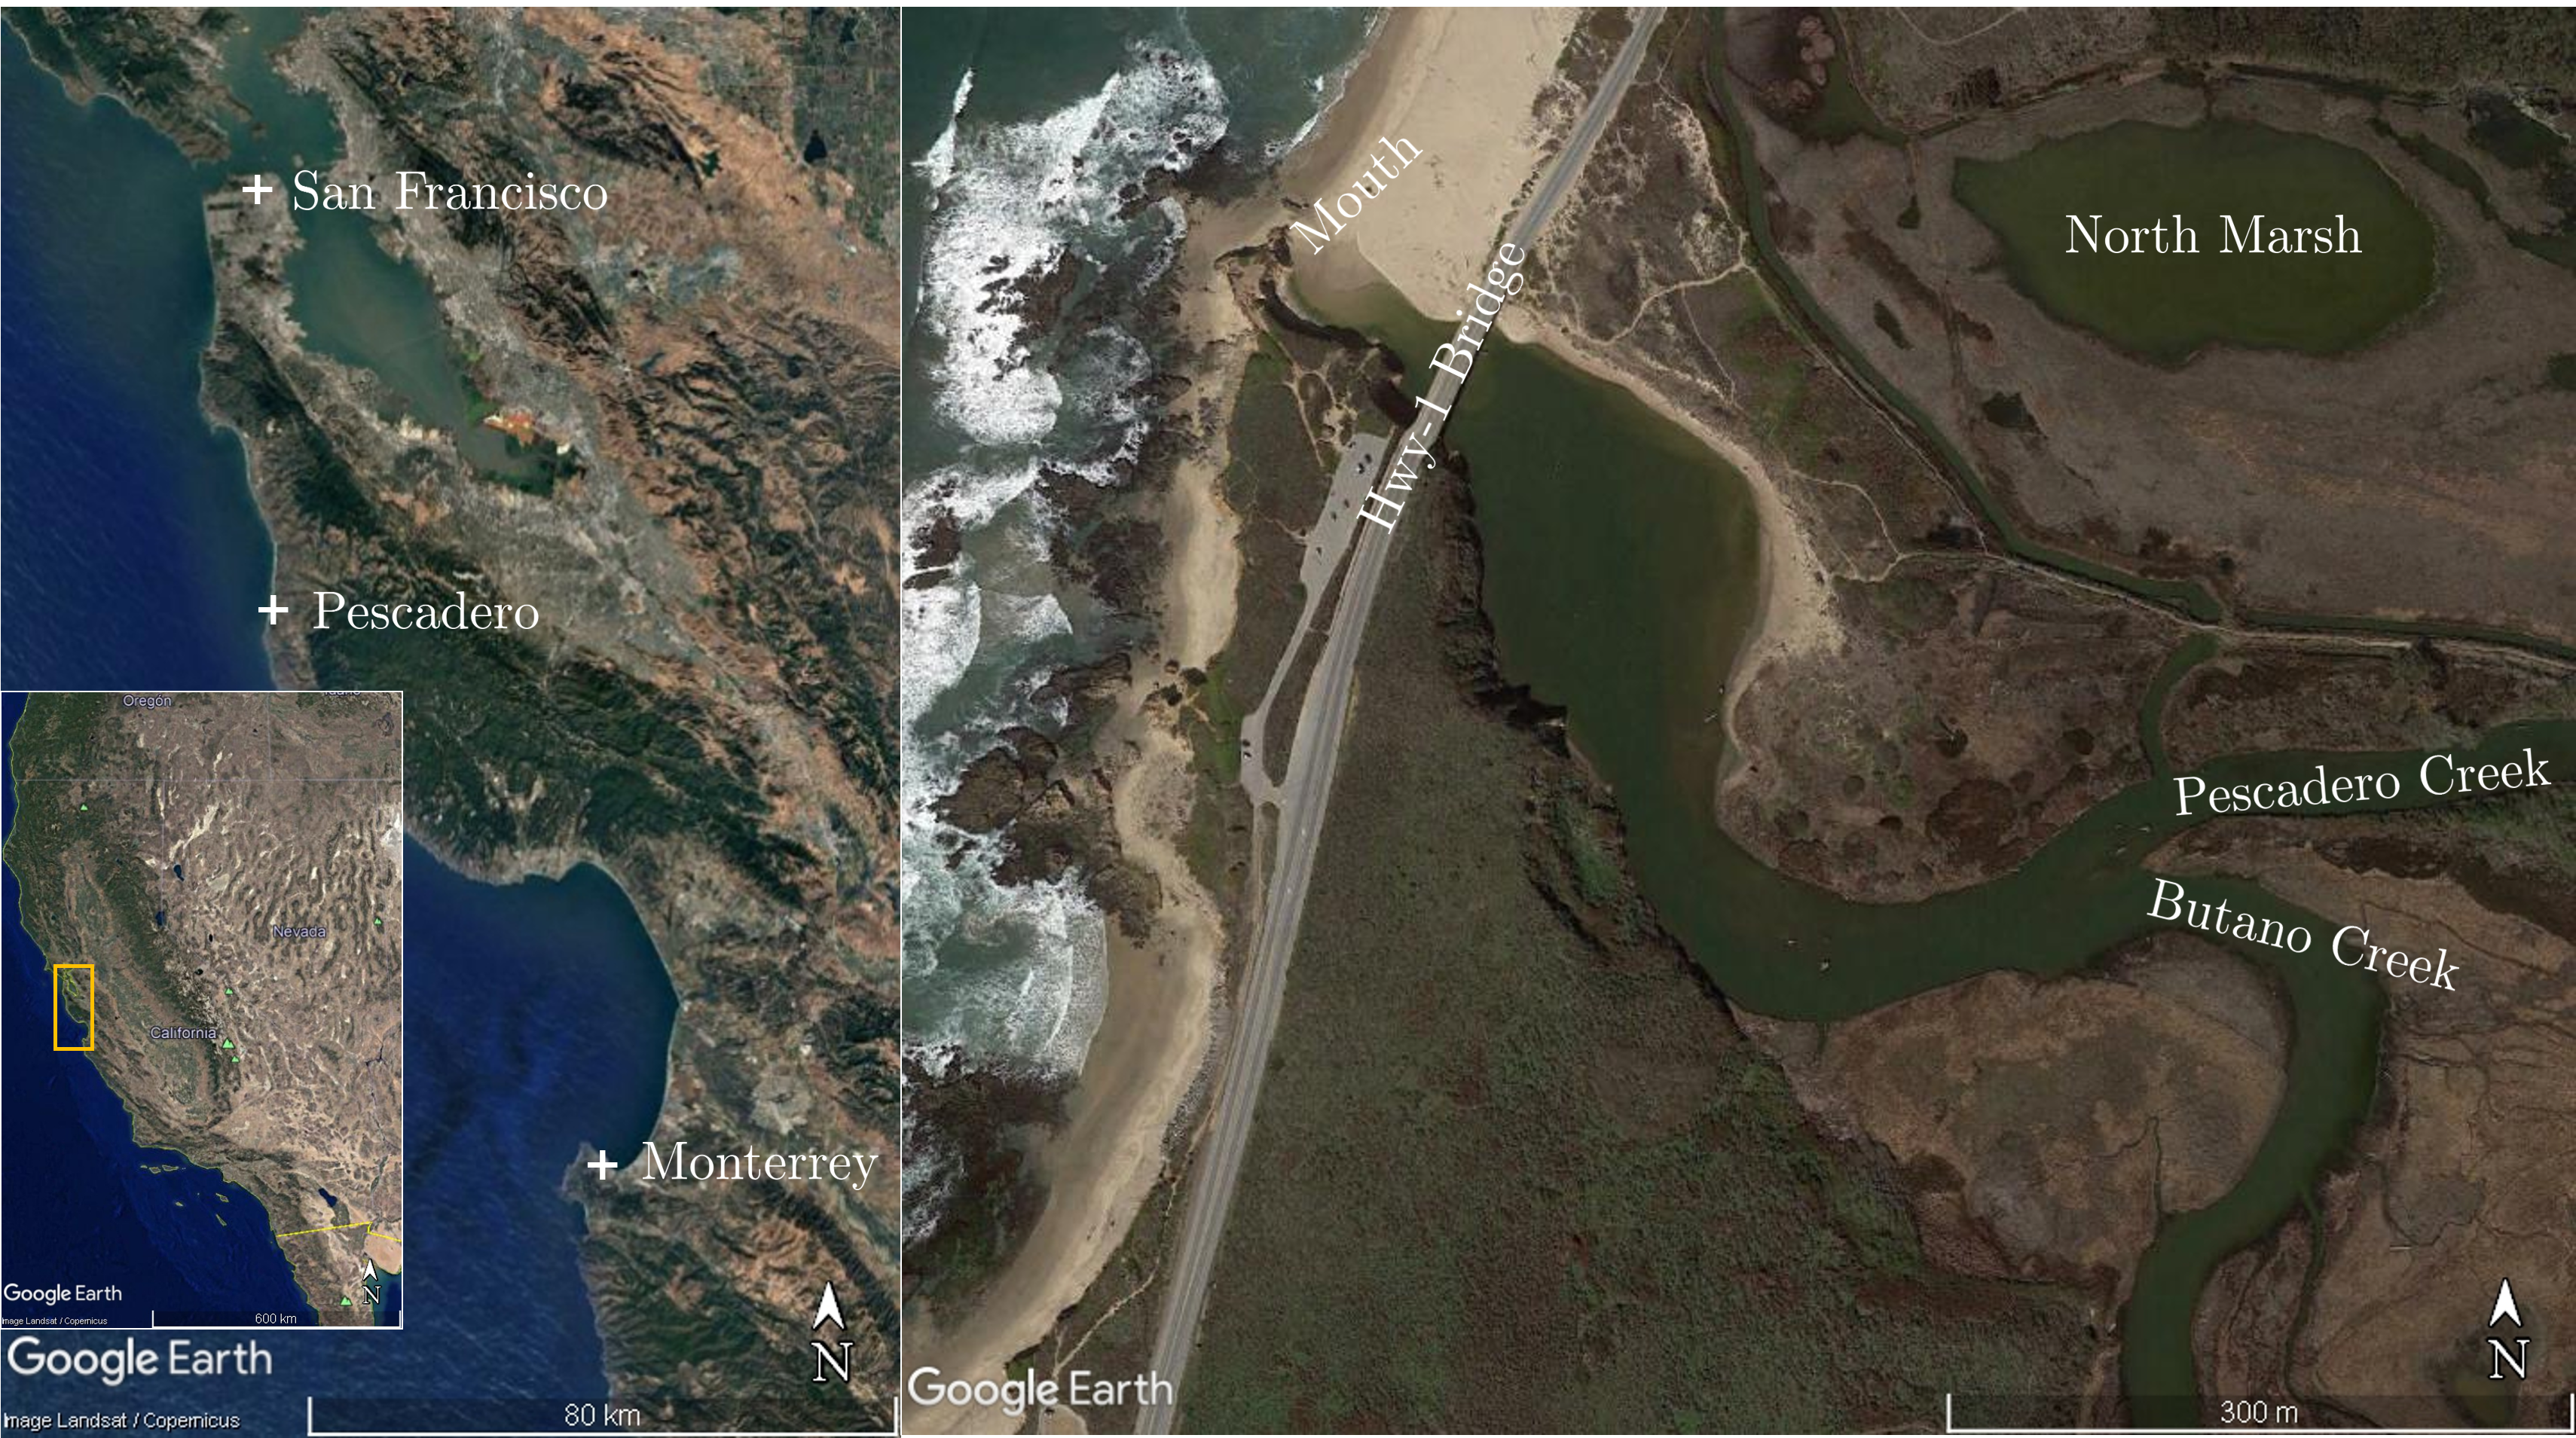
\includegraphics[scale=0.6]{Imagenes/mapa1.png}
\caption{Location of Pescadero Estuary on California's Coastline. Images reprocessed from Google Earth.}
\label{fig:locPDO}
\end{figure}

The sand barrier placed at the inlet of Pescadero closes the estuary from the sea, changing its behavior to a stratified lagoon which usually happens during the dry season \citep{Williams2014}. Inlet rupture usually occurs during the wet season when precipitation increases flow and the lagoon fills to overflowing, leading to the scour of a new channel between the lagoon and the return of tidal action and seawater intrusions to the estuary \citep{largier2015}. During periods when the mouth of the estuary is closed, the water level of the lagoon rises and could flood the surrounding marshy land. \\

The significance of this site lies in the detection of fish kills after the breaching of the lagoon mouth after an extended closure \citep{largier2015}. Also, there are agricultural lands on the surroundings that have a productive importance for the local community in addition to other concerns as winter flooding of low-lying lands, in which exists some roads and parts of the town, or the presence of a wide diversity of habitats and microhabitats in the estuary.\\

Pescadero has two main water inputs: freshwater inflow and saline water, which sometimes get mixed and other times form a two-layer structure. The behavior of the estuary depends on the mouth state, where we can observe an 'open' and 'closed' state. Pescadero receives freshwater inflow from two relatively small watersheds, which have a highly variable discharge, following precipitation that varies from day to day through the wet season, as well as seasonally and between years \citep{largier2015}. The Pescadero watershed is about twice the size of the Butano watershed, and produces 57\% of the streamflow \citep{Williams2014}. On the other hand the Northern Californian coast experiences a semidiurnal tide with a neap tide range of under 1 m and a spring tide range up to almost 3 m \citep{Williams2014}. Saltwater get into the estuary easily during open state, but when the inlet is closed seawater has to overtop the sandbar to get into the estuary, which happens occasionally during high tide and strong waves.\\

When the mouth is closed the estuary takes a stratified structure fed by the freshwater input and the sporadic wave overtopping saline water. In this form is more difficult to energize the water column, but it can happen with external factors as wind stress in the surface or from the discharge and the wave overtopping. However, vertical transport in Pescadero couldn't be from density-driven exchange, because the estuary would be always saltier than the creeks input water, so it always will stay on the top of the water column making the estuary stratified. Even that, in Pescadero there is a light density/salinity gradient due to the freshwater input upstream and the saltwater overtopping the bar at the other end.\\

\subsection{Motivation}

In its state of disconnection from the ocean (i.e., closed state), the estuary can take the form of a shallow stratified lagoon, due to the presence of saltwater and freshwater from fluvial inputs \citep{Behrens2016}. This estuary state could lead to eutrophication if there are no energy inputs to the system \citep{nunes2014responses}, and usually, the wind is the main source, driving to mixing and destratification in small bar-built estuaries \citep{Gale2006} triggering processes that impact mixing and circulation, which could affect the marine life of the estuary \citep{marti2008relating}. \\

As said before, the wind is the principal driver of mixing present, but sometimes stratification makes difficult to energize the denser layer, leading in some cases to suppression of turbulence below the pycnocline \citep{Cousins2010}. This could cause hypoxia or anoxia in the lower layers \citep{Kelly2018} or retention of nutrients in the bottom \citep{Cousins2010} and when there is upwelling or mixing, abrupt changes could occur for marine life and generate problems or even death \citep{marti2008relating}.\\  

Due to the latter, these waterbodies are highly dynamic, and this makes them sites of great importance for research. On the other hand, estuaries are the connection between the earth and the ocean, receiving waters coming from rivers and creeks that are exposed to anthropogenic effects, causing changes in freshwater flow or temperature, in addition, to being subjected to sea level rise and wave climate variations \citep{grez2020evidence, holt2010potential, thorne2021wetlands}. Besides, in the estuaries, of their contact with the coast and rivers, activities such as fish farming or agriculture are developed, so they have economic and social importance to communities. \\

The response to strong and sustained wind stress in a closed state bar-built estuary starts with a setup of the surface and a change in the pressure gradient. This will cause the pycnocline to tilt upwards at the upwind end of the estuary leading sometimes the bottom layers to rise to the surface. The reduction or end of this wind forcing releases the pycnocline from its tilted position and return to horizontal. The upwelling effect caused by wind forcing has potential relevance in nutrient and oxygen exchange between layers \citep{Kelly2018} and has been studied widely in lakes using temperature measurements \citep{Coman2012, delafuente2010strong, roberts2021setup}, however, there are fewer studies that observe this kind of behavior at bar-built estuaries or in smaller coastal lagoons. \\

\end{document}